
\section{Methods}

The development of the fully featured COMBINE archive can be divided into three major parts.
I first decided for a simulation study to encode in an archive, then I created an initial archive which was then enriched with information I found on the internet and data that I generated on my own.
These steps are described in the following.

\subsection{Deciding for a Simulation Study}

I developed 3 criteria to decide for a simulation study:

\paragraph{Criteria 1: Open Access.}
As I want to share the demo archive openly, I had to decide for an experiment that offers as much open data as possible.
Obviously and unfortunately, the publication, as an essential document for the documentation of experiments, is the bottleneck.
Therefore, I needed to find a simulation experiment which was published using an open access license.

\paragraph{Criteria 2: Much data already available in standard formats.}
As I did not want to encoded the model myself, I restricted my search to studies which are already available as SBML and CellML models.
Ideally, these models are already curated, which increases my trust in the encoding.

\paragraph{Criteria 3: I have ideally already dealt with that publication.}
As I will need to work with the study I need to understand it.
It usually takes a lot of time to dig into a new field, so I preferred studies that I already investigated.
However, this was just a soft criteria to decrease my workload.


\paragraph{Searching for a matching study.}
Searching for a study was harder than I thought.
I failed to encoded my search criteria for the search engines of current databases.
I ended up asking a common search engine to look for names of open access journals at the websites of the databases and eventually \texttt{site:models.cellml.org "Molecular Systems Biology"}\footnote{\href{https://duckduckgo.com/?q=site\%3Amodels.cellml.org+\%22Molecular+Systems+Biology\%22}{duckduckgo.com/?q=site\%3Amodels.cellml.org+\%22Molecular+Systems+Biology\%22}} resulted in a model that is available from the CellML model repository (Calzone, Thieffry, Tyson, Novak, 2007\footnote{\href{http://models.cellml.org/exposure/1a3f36d015121d5596565fe7d9afb332}{models.cellml.org/exposure/1a3f36d015121d5596565fe7d9afb332}}) \cite{cellmlrepo} and from the Biomodels Database (BIOMD0000000144\footnote{\href{http://www.ebi.ac.uk/biomodels-main/BIOMD0000000144}{www.ebi.ac.uk/biomodels-main/BIOMD0000000144}}) \cite{biomodels}.


\paragraph{The final study.}
The study I chose was published by Calzone \emph{et.~al.} in Molecular Systems Biology. They propose a dynamical model for the molecular events underlying rapid, synchronous, syncytial nuclear division cycles in \textit{Drosophila} embryos \cite{Calzone2007}.
In an earlier study dealing with the cell cycle I already touched that publication, so it was the perfect study for the demo archive project.




\subsection{Creating an initial COMBINE archive}

\begin{figure}
\begin{center}
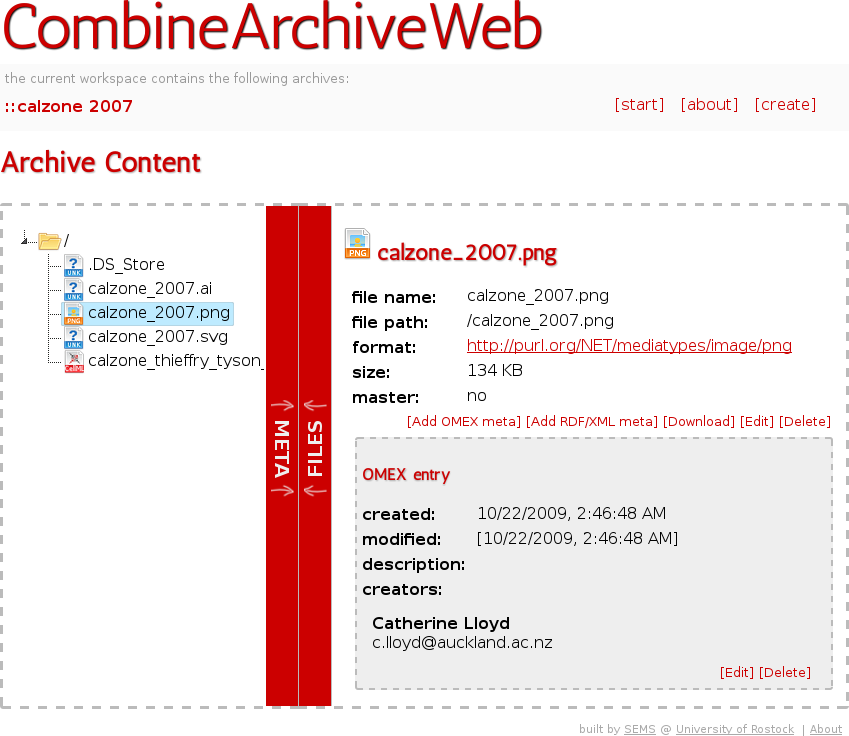
\includegraphics[width=.8\textwidth]{img/webcat-screenshot-combined.png}
\end{center}
\caption{The CombineArchiveWeb application showing the archive as it was exported from M2CAT. The files were cloned from the CellML model repository and immediately annotated with meta data. Thus, it is clear that I am not the creator of \textit{calzone\_2007.png}, instead it lists Catherine Lloyd as the creators and .}
\label{fig:screen:webcat}
\end{figure}

I created an initial version of the COMBINE archive using M2CAT \cite{m2cat}.
The webinterface as \href{http://m2cat.sems.uni-rostock.de/}{m2cat.sems.uni-rostock.de} searches in a graph database to retrieve links to models published in open databases \cite{masymos}.
The search for \texttt{Calzone} resulted in two matches, one of them representing the model in the CellML model repository.
In addition to searching in a graph database, M2CAT is also able to retrieve the files that correspond to a simulation study from other sources, such as open model repositories, and to bundle them in combine archives using the library of the CombineArchive Toolkit \cite{cat}.
The web interface also provides means to immediately explore the generated archive in the CombineArchiveWeb application \cite{scharm2014}.

In case of the Calzone \emph{et.~al.} study, the files of the CellML model repository were cloned and aggregated in a new COMBINE archive.
Additionally, the resulting archive and its files were annotated with all the meta data available from the GIT project of the CellML model repositories.
Specifically, the archive was annotated with the information that it was generated by M2CAT, and the files that were cloned from the CellML model repository are annotated with creators/contributors and modification times as available from the corresponding GIT project (\texttt{git log}), see Figure~\ref{fig:screen:webcat}. Thus, the an initial version of the COMBINE archive was obtained automatically and very quickly.






\subsection{Extending the COMBINE archive}
As the initial version only contains the model encoded in CellML together with some figures (all files exclusively from the CellML model repository) I needed to extend the archive manually.
To organize the files I developed a structure containing the following directories:
\begin{itemize}
 \item \texttt{model/}: files that encode an visualise the biological system
 \item \texttt{experiment/}: files that encode the \textit{in silico} setup of the experiment
 \item \texttt{documentation/}: files that describe and document the model and/or experiment
 \item \texttt{result/}: files that result from running the experiment
\end{itemize}

Using the CombineArchiveWeb application it was very easy to get rid of the unrelated \texttt{.DS\_Store} file. In the web interface I also moved all other files into the model directory, as they all encoded the mode.
The other directories are to be filled in the next sections.

\subsubsection{Retrieving Data and Information from other Services}
The first chapter of extending the archive dealt with a search for resources related to this study on the internet.

\paragraph{The article} is usually the central object of a research study. As I said earlier, Calzone \emph{et.~al.} published their findings in Molecular Systems Biology. So I went to the corresponding website\footnote{\href{http://msb.embopress.org/content/3/1/131}{msb.embopress.org/content/3/1/131}} and downloaded the article and supplementary information.
As both describe the experiment, I uploaded the files to the documentation directory in the CombineArchiveWeb application.
The web interface decently added meta data listing me as the creator of the file, which, unfortunately, is in this case incorrect.
Thus, I modified the entry to attribute the real creators.
Additionally, I also added modification dates to the meta data of these files by copying them from the website of the article and the meta data of the PDF.
The CombineArchiveWeb application provides a nice interface to modify the meta data without knowledge about XML or RDF.
However, in the background it created a RDF/XML tree to describe the main article and added it to the meta data file of the archive, see section~\ref{sec:rdfmeta}.



download
supp
upload
recreated meta data


seek for more information on that model
and add that to the archive

\subsubsection{Generating more Data}
creating simulation description
simulating it
storing results

generating sbgn compliant figure



